\chapter{कार्बनिक रसायन में ऑक्सीकरण और अपचयन}\label{ch:b1:organic-redox}

खुली छोड़ी गई वाइन की बोतल कुछ ही दिनों में सिरके में बदल जाती है: जीवाणु
वायु की ऑक्सीजन से एथेनॉल को एथेनोइक अम्ल में ऑक्सीकृत कर देते हैं। कोई कीटोन और
वह ऐल्कोहॉल जिससे वह आता है, दो हाइड्रोजन परमाणुओं से भिन्न होते हैं --- और, ठीक से
गिनें तो, दो इलेक्ट्रॉनों से। कार्बनिक ऑक्सीकरण और अपचयन
\cref{ch:b1:nernst} के धातु आयनों के बीच इलेक्ट्रॉनों के विनिमय जैसे नहीं दिखते,
क्योंकि इलेक्ट्रॉन प्रोटॉनों के साथ या हाइड्राइड आयनों के साथ यात्रा करते हैं, पर
लेखा-जोखा वही है। यह अध्याय कार्बन को \omterm{def:b1:organic-redox:oxidation-level}{ऑक्सीकरण स्तर} देता है,
उनसे यह पूर्वानुमान करता है कि ऑक्सीकृत होने पर हर ऐल्कोहॉल क्या देता है, और
कार्बोनिल यौगिकों को अपचित करने वाले हाइड्राइड अभिकर्मकों का परिचय देता है,
इस पर ध्यान रखते हुए कि हर अभिकर्मक किन समूहों को अछूता छोड़ देता है।

\begin{recall}
\omterm{def:b1:nernst:oxidation-number}{ऑक्सीकरण संख्याएँ}, \omterm{def:b1:nernst:couple}{अर्ध-समीकरण} और अपचयोपचय समीकरणों का संतुलन
\cref{ch:b1:nernst} में हैं; ऐल्कोहॉलों और कार्बनों की श्रेणियाँ
\cref{ch:b1:electronic-effects} में; \omterm{def:b1:acetals-protection:hemiacetal}{ऐसीटैल} और कार्बोनिल
समूहों का \omterm{def:b1:acetals-protection:protecting-group}{रक्षण} \cref{ch:b1:acetals-protection} में; ग्रीन्यार योग
\cref{ch:b1:organomagnesium} में।
\end{recall}

\begin{omfigure}
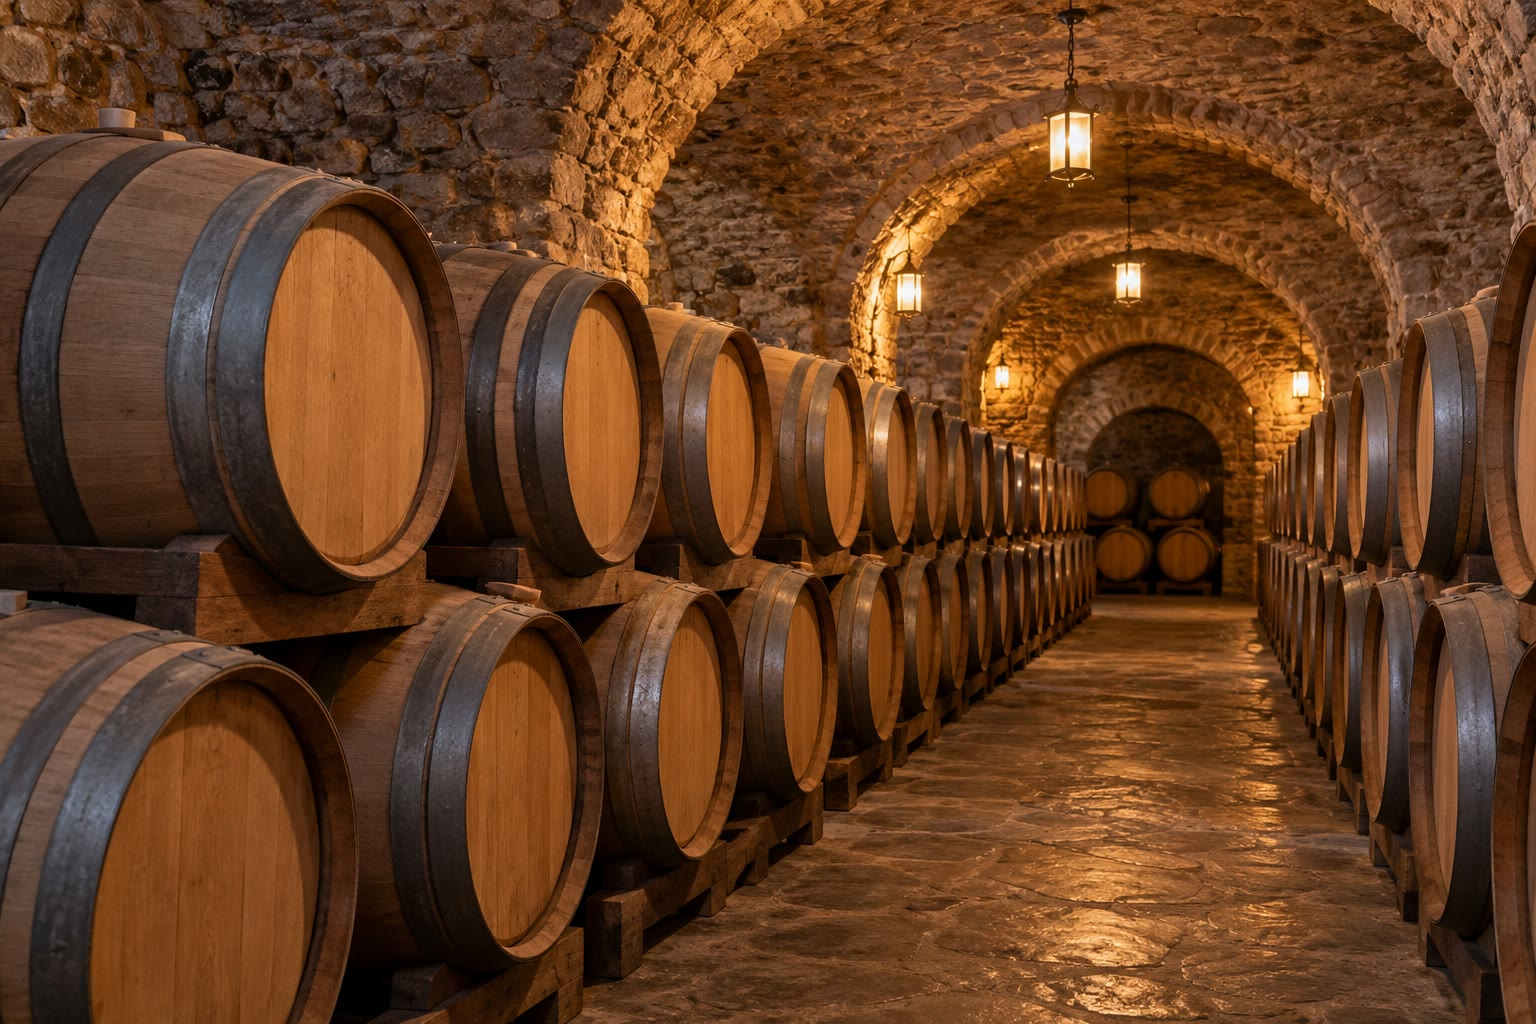
\includegraphics[width=0.58\linewidth]{images/book2/ai/b1-24-wine-cellar.jpg}

{\small तहख़ाने में परिपक्व होती वाइन। वायु से बचाकर रखने पर वाइन अपना एथेनॉल बनाए रखती है;
वायु के संपर्क में, ऐसीटिक अम्ल जीवाणु उसे एथेनोइक अम्ल में ऑक्सीकृत कर देते हैं।}
\end{omfigure}

\section{कार्बन के ऑक्सीकरण स्तर}

\begin{definition}[ऑक्सीकरण स्तर]\label{def:b1:organic-redox:oxidation-level}
किसी कार्बन परमाणु का \emph{ऑक्सीकरण स्तर}\index{ऑक्सीकरण स्तर} उसकी
\omterm{def:b1:nernst:oxidation-number}{ऑक्सीकरण संख्या} है, जो \cref{prop:b1:nernst:on-rules} के नियमों से
प्राप्त होती है: किसी अधिक विद्युत-ऋणात्मक परमाणु (O, N, हैलोजन) से हर आबंध
$+1$ गिना जाता है, हाइड्रोजन से हर आबंध $-1$, और किसी
अन्य कार्बन से हर आबंध 0 (द्वि-आबंध दो बार गिना जाता है)।
\end{definition}

\begin{proposition}[कार्बन की ऑक्सीकरण संख्याएँ]\label{prop:b1:organic-redox:on-of-carbon}
किसी कार्बन की \omterm{def:b1:nernst:oxidation-number}{ऑक्सीकरण संख्या} (O, N या हैलोजनों से आबंधों की संख्या)
घटा (H से आबंधों की संख्या) के बराबर है। समान कार्बन कंकाल वाले यौगिकों के
एक ही कुल में, ऐल्कोहॉल $\to$ ऐल्डिहाइड या कीटोन $\to$
कार्बोक्सिलिक अम्ल $\to$ कार्बन डाइऑक्साइड ऑक्सीकरणों की एक शृंखला है, हर एक दो
इलेक्ट्रॉनों का।
\end{proposition}

\begin{proof}
हर आबंध तोड़कर दोनों इलेक्ट्रॉन अधिक विद्युत-ऋणात्मक
भागीदार को देने पर: H से (जो C से कम विद्युत-ऋणात्मक है) कार्बन एक इलेक्ट्रॉन पाता है,
प्रति C--H आवेश $-1$; O, N, हैलोजनों (जो अधिक विद्युत-ऋणात्मक हैं) को वह एक
खोता है, प्रति आबंध $+1$; C--C आबंध बराबर बाँटे जाते हैं। \ce{-CH2OH}
(एक अन्य कार्बन से आबंधित कार्बन के लिए $-1$) से \ce{-CHO} ($+1$) से
\ce{-COOH} ($+3$) तक जाने पर, संख्या हर चरण में 2 बढ़ती है: दो इलेक्ट्रॉन।
\end{proof}

\begin{omfigure}
\begin{tikzpicture}[font=\small, >={Stealth}]
  \foreach \x/\f/\n in {0/\ce{CH4}/-4, 2.4/\ce{CH3OH}/-2, 4.8/\ce{HCHO}/0, 7.2/\ce{HCOOH}/+2, 9.6/\ce{CO2}/+4} {
    \node[draw, rounded corners, minimum width=1.5cm] at (\x,0) {\f};
    \node[below] at (\x,-0.5) {$\n$};
  }
  \foreach \x in {0.8,3.2,5.6,8.0} \draw[->, thick, omThm] (\x,0) -- ++(0.8,0);
  \node[omThm, above] at (4.8,0.5) {ऑक्सीकरण: हर चरण में $-2\,\mathrm{e^-}$ (और $-2\,\ce{H+}$)};
  \node[left] at (-0.9,-0.75) {C की ऑक्सीकरण संख्या:};
\end{tikzpicture}

{\small एक-कार्बन कुल के \omterm{def:b1:organic-redox:oxidation-level}{ऑक्सीकरण स्तर}: मेथेन, मेथेनॉल,
मेथेनल, मेथेनोइक अम्ल, कार्बन डाइऑक्साइड। हर तीर दो-इलेक्ट्रॉन
ऑक्सीकरण है; उलटा पढ़ें तो एक अपचयन।}
\end{omfigure}

\begin{method}[किसी कार्बनिक अर्ध-समीकरण को संतुलित करना]\label{met:b1:organic-redox:balance-organic-redox}
\begin{enumerate}
  \item समान कंकाल वाले कार्बनिक \omterm{def:b1:nernst:couple}{ऑक्सीकारक} और \omterm{def:b1:nernst:couple}{अपचायक} लिखिए।
  \item बदलने वाले कार्बनों की \omterm{def:b1:nernst:oxidation-number}{ऑक्सीकरण संख्याओं} के परिवर्तन से
        इलेक्ट्रॉन गिनिए (या सरलता से: खोए गए H के हर युग्म के लिए, या प्राप्त हर O के लिए,
        दो)।
  \item ऑक्सीजन को जल से, हाइड्रोजन को \ce{H+} से, आवेश को
        इलेक्ट्रॉनों से संतुलित कीजिए।
\end{enumerate}
एथेनॉल से एथेनोइक अम्ल: \ce{CH3CH2OH + H2O -> CH3COOH + 4H+ + 4e-}।
अम्लीकृत डाइक्रोमेट (\ce{Cr2O7^2- + 14H+ + 6e- -> 2Cr^3+ + 7H2O}) के साथ,
दो डाइक्रोमेट आयनों के लिए एथेनॉल के तीन अणु:
\ce{3CH3CH2OH + 2Cr2O7^2- + 16H+ -> 3CH3COOH + 4Cr^3+ + 11H2O}।
\end{method}

\section{ऐल्कोहॉलों का ऑक्सीकरण}

\begin{proposition}[ऑक्सीकृत होने पर ऐल्कोहॉल क्या देते हैं]\label{prop:b1:organic-redox:alcohol-oxidation}
प्राथमिक ऐल्कोहॉल \ce{RCH2OH} ऐल्डिहाइड \ce{RCHO} में ऑक्सीकृत होता है, फिर
(जल में, प्रबल \omterm{def:b1:nernst:couple}{ऑक्सीकारक} के साथ) कार्बोक्सिलिक अम्ल \ce{RCOOH} में;
द्वितीयक ऐल्कोहॉल \ce{R2CHOH} कीटोन \ce{R2CO} में, जो आगे के
ऑक्सीकरण का प्रतिरोध करता है; तृतीयक ऐल्कोहॉल \ce{R3COH} किसी C--C आबंध को
तोड़े बिना ऑक्सीकृत नहीं होता।
\end{proposition}

\begin{proof}
ऐल्कोहॉल का ऑक्सीकरण OH का हाइड्रोजन और कार्बिनॉल कार्बन से एक
हाइड्रोजन हटाता है, जिससे C=O बनता है। तृतीयक कार्बिनॉल कार्बन पर ऐसा कोई
हाइड्रोजन नहीं होता। ऐल्डिहाइड के कार्बोनिल कार्बन पर अब भी एक H है;
जल में वह आंशिक रूप से जलयोजित होता है, \ce{RCH(OH)2}, जो फिर उसी ढंग से
ऑक्सीकृत होकर \ce{RCOOH} बनता है। कीटोन के उस कार्बन पर कोई H नहीं होता और वह रुक जाता है।
\end{proof}

जल में प्रबल \omterm{def:b1:nernst:couple}{ऑक्सीकारक} --- अम्लीकृत पोटैशियम डाइक्रोमेट या
परमैंगनेट --- प्राथमिक ऐल्कोहॉलों को अम्लों तक ऑक्सीकृत करते हैं।
ऐल्डिहाइड पर रुकने के लिए, उसे बनते ही आसवित करके निकाल लिया जाता है (ऐल्डिहाइड
जिन ऐल्कोहॉलों से आते हैं उनसे कम ताप पर उबलते हैं, क्योंकि उनमें O--H \omterm{def:b1:intermolecular-forces-solvents:hbond}{हाइड्रोजन आबंध} नहीं होते), या
द्वितीय वर्ष के खंड में वर्णित मृदु, निर्जल अभिकर्मक प्रयुक्त किए जाते हैं।

\begin{safety}{\ghs[5mm]{GHS03}\,\ghs[5mm]{GHS05}\,\ghs[5mm]{GHS06}\,\ghs[5mm]{GHS07}\,\ghs[5mm]{GHS08}\,\ghs[5mm]{GHS09}}
पोटैशियम डाइक्रोमेट, ऐल्कोहॉलों का पारंपरिक नारंगी \omterm{def:b1:nernst:couple}{ऑक्सीकारक},
उन पदार्थों में वर्गीकृत है जो कैंसर उत्पन्न कर सकते हैं: उसे केवल
थोड़ी मात्रा में, दस्तानों और चश्मे के साथ, संभाला जाता है, और उसका क्रोमियम अपशिष्ट
अलग से एकत्रित किया जाता है; जहाँ संभव हो, कम संकटमय \omterm{def:b1:nernst:couple}{ऑक्सीकारक} को
वरीयता दी जाती है।
% ledger: ghs:K2Cr2O7
\end{safety}

\section{हाइड्राइडों द्वारा कार्बोनिल यौगिकों का अपचयन}

\begin{definition}[हाइड्राइड दाता]\label{def:b1:organic-redox:hydride-donor}
\emph{हाइड्राइड दाता}\index{हाइड्राइड दाता} एक हाइड्रोजन परमाणु को
उसके \omterm{def:b1:lewis-resonance-vsepr:lewis}{आबंधी युग्म} सहित, \ce{H-}, किसी \omterm{def:b1:electronic-effects:nucleophile}{इलेक्ट्रॉनरागी} कार्बन को स्थानांतरित करता है। सोडियम बोरोहाइड्राइड
\ce{NaBH4} और लिथियम ऐलुमिनियम हाइड्राइड \ce{LiAlH4} \emph{संकुल
धातु हाइड्राइड}\index{संकुल धातु हाइड्राइड} हैं: हाइड्राइड
\ce{BH4-} या \ce{AlH4-} आयन से पहुँचाया जाता है, मुक्त आयन के रूप में नहीं।
\end{definition}

\begin{omfigure}
\setchemfig{atom sep=2.1em}
\schemestart
\chemfig{H_3B^{-}-[@{bh}]@{h}H}
\+
\chemfig{@{c}C(-[:150]R)(-[:210]R')=[@{co}]@{o}O}
\arrow{->}
\chemfig{C(-[:150]R)(-[:210]R')(-[2]H)-O^{-}}
\arrow{->[\ce{H2O}]}
\chemfig{C(-[:150]R)(-[:210]R')(-[2]H)-OH}
\schemestop
\chemmove{\draw[->, thick, shorten <=2pt, shorten >=3pt](bh) .. controls +(80:9mm) and +(180:7mm) .. (c);
          \draw[->, thick, shorten <=2pt, shorten >=2pt](co) .. controls +(90:6mm) and +(90:6mm) .. (o);}
\par\vspace{6pt}

{\small बोरोहाइड्राइड द्वारा किसी कीटोन का अपचयन: एक B--H युग्म नया C--H
आबंध बनाता है जबकि C=O का $\pi$ युग्म ऑक्सीजन पर जाता है; \omterm{def:b1:alcohol-activation:alkoxide}{ऐल्कॉक्साइड}
विलायक (जल या कोई ऐल्कोहॉल) द्वारा या उपचार के समय प्रोटॉनित होता है। हर \ce{BH4-}
अपने चारों हाइड्रोजन बारी-बारी से पहुँचा सकता है।}
\end{omfigure}

\begin{proposition}[दोनों हाइड्राइडों का कार्यक्षेत्र]\label{prop:b1:organic-redox:hydride-scope}
सोडियम बोरोहाइड्राइड, जल या ऐल्कोहॉलों में प्रयुक्त, ऐल्डिहाइडों को
प्राथमिक ऐल्कोहॉलों में और कीटोनों को द्वितीयक ऐल्कोहॉलों में अपचित करता है, और एस्टरों,
कार्बोक्सिलिक अम्लों, ऐमाइडों और C=C द्वि-आबंधों को अछूता छोड़ देता है। लिथियम
ऐलुमिनियम हाइड्राइड, शुष्क ईथर में प्रयुक्त, एस्टरों और कार्बोक्सिलिक
अम्लों को भी प्राथमिक ऐल्कोहॉलों में अपचित करता है, और जल से प्रचंड अभिक्रिया करता है।
\end{proposition}

\begin{proof}
Al--H आबंध B--H आबंध से अधिक ध्रुवित है (ऐलुमिनियम बोरॉन से कम
विद्युत-ऋणात्मक है), इसलिए \ce{AlH4-} कहीं अधिक प्रबल \omterm{def:b1:organic-redox:hydride-donor}{हाइड्राइड
दाता} है, जो एस्टरों और
कार्बोक्सिलेटों के कम \omterm{def:b1:electronic-effects:nucleophile}{इलेक्ट्रॉनरागी} कार्बोनिल पर आक्रमण कर सकता है; यही अभिक्रियाशीलता उसे किसी भी अम्लीय
हाइड्रोजन से, जल सहित, अभिक्रिया करवाती है। \ce{BH4-} जल और
ऐल्कोहॉलों से केवल धीरे अभिक्रिया करता है, और केवल सबसे \omterm{def:b1:electronic-effects:nucleophile}{इलेक्ट्रॉनरागी} कार्बोनिलों पर आक्रमण करता है। एक पृथक
C=C आबंध \omterm{def:b1:electronic-effects:nucleophile}{इलेक्ट्रॉनरागी} नहीं है और दोनों में से कोई उसे अपचित नहीं करता।
\end{proof}

\section{वरणात्मकता}

\begin{definition}[रसायनवरणात्मक अभिक्रिया]\label{def:b1:organic-redox:chemoselective}
\emph{रसायनवरणात्मक अभिक्रिया}\index{रसायनवरणात्मक अभिक्रिया} किसी अणु के
एक क्रियात्मक समूह पर ऐसे अन्य समूहों की उपस्थिति में कार्य करती है जो
किसी अन्य अभिकर्मक के साथ, अभिक्रिया भी कर सकते थे।
\end{definition}

\begin{omfigure}
\begin{tabular}{lcc}
\hline
समूह & \ce{NaBH4} (ऐल्कोहॉल विलायक) & \ce{LiAlH4} (शुष्क ईथर) \\
\hline
ऐल्डिहाइड \ce{RCHO} & प्राथमिक ऐल्कोहॉल & प्राथमिक ऐल्कोहॉल \\
कीटोन \ce{R2CO} & द्वितीयक ऐल्कोहॉल & द्वितीयक ऐल्कोहॉल \\
एस्टर \ce{RCOOR} & कोई अभिक्रिया नहीं & दो ऐल्कोहॉल \\
कार्बोक्सिलिक अम्ल \ce{RCOOH} & कोई अभिक्रिया नहीं (लवण) & प्राथमिक ऐल्कोहॉल \\
ऐल्कीन \ce{C=C} & कोई अभिक्रिया नहीं & कोई अभिक्रिया नहीं \\
\omterm{def:b1:acetals-protection:hemiacetal}{ऐसीटैल} & कोई अभिक्रिया नहीं & कोई अभिक्रिया नहीं \\
\hline
\end{tabular}

\smallskip
{\small दोनों हाइड्राइड क्या अपचित करते हैं। सोडियम बोरोहाइड्राइड
रसायनवरणात्मक अभिकर्मक है; लिथियम ऐलुमिनियम हाइड्राइड, शक्तिशाली अभिकर्मक।}
\end{omfigure}

\begin{example}[एक कीटो एस्टर]\label{ex:b1:organic-redox:ketoester}
एथिल 4-ऑक्सोपेंटेनोएट, \ce{CH3CO(CH2)2COOEt}, सोडियम बोरोहाइड्राइड के साथ
एथिल 4-हाइड्रॉक्सीपेंटेनोएट देता है: केवल कीटोन अपचित होता है। लिथियम
ऐलुमिनियम हाइड्राइड के साथ दोनों समूह अपचित होते हैं: पेंटेन-1,4-डाइऑल (और
एथेनॉल)। केवल एस्टर को अपचित करने के लिए, कीटोन का पहले
\omterm{def:b1:acetals-protection:hemiacetal}{ऐसीटैल} के रूप में \omterm{def:b1:acetals-protection:protecting-group}{रक्षण} करना होगा (\cref{ch:b1:acetals-protection})।
\end{example}

\begin{inthelab}[किसी कीटोन का अपचयन]
सोडियम बोरोहाइड्राइड को एथेनॉल में कीटोन के ठंडे विलयन में छोटे-छोटे भागों में
मिलाया जाता है: अभिक्रिया ऊष्माक्षेपी है, और विलायक के साथ अभिकर्मक की
धीमी अभिक्रिया से हाइड्रोजन के बुलबुले निकलते हैं। विलोडन के बाद, तनु
अम्ल आधिक्य अभिकर्मक को नष्ट करता है (और हाइड्रोजन: पास में कोई लौ नहीं) और
ऐल्कोहॉल का निष्कर्षण किया जाता है। इसके विपरीत, लिथियम ऐलुमिनियम हाइड्राइड केवल
अक्रिय गैस के अंतर्गत शुष्क ईथर में प्रयुक्त होता है, और उसका आधिक्य
अत्यंत सावधानी से नष्ट किया जाता है।
\end{inthelab}

\section{अभ्यास}

\begin{exercise}[$\star$]\label{exo:b1:organic-redox:1}
एथेनॉल, एथेनल, एथेनोइक
अम्ल, प्रोपेनोन और मेथेनोइक अम्ल में हर कार्बन की \omterm{def:b1:nernst:oxidation-number}{ऑक्सीकरण संख्या} बताइए।
\end{exercise}

\begin{exercise}[$\star$]\label{exo:b1:organic-redox:2}
अम्लीकृत डाइक्रोमेट प्रोपेन-1-ऑल, प्रोपेन-2-ऑल और
2-मेथिलप्रोपेन-2-ऑल के साथ क्या देता है?
\end{exercise}

\begin{exercise}[$\star$]\label{exo:b1:organic-redox:3}
अम्ल में युग्मों प्रोपेनोन/प्रोपेन-2-ऑल और
एथेनल/एथेनॉल के \omterm{def:b1:nernst:couple}{अर्ध-समीकरण} लिखिए।
\end{exercise}

\begin{exercise}[$\star$]\label{exo:b1:organic-redox:4}
सोडियम बोरोहाइड्राइड और लिथियम ऐलुमिनियम हाइड्राइड
ब्यूटेनल, ब्यूटेनोन, एथिल ब्यूटेनोएट और ब्यूटेनोइक अम्ल के साथ क्या देते हैं?
\end{exercise}

\begin{exercise}[$\star\star$]\label{exo:b1:organic-redox:5}
अम्ल में परमैंगनेट (\ce{MnO4-}/\ce{Mn^2+}) द्वारा प्रोपेन-2-ऑल के ऑक्सीकरण को संतुलित कीजिए
और \qty{1.20}{g} ऐल्कोहॉल ($M = \qty{60.0}{g/mol}$) के लिए आवश्यक
\qty{0.020}{mol/L} परमैंगनेट का आयतन परिकलित कीजिए।
\end{exercise}

\begin{exercise}[$\star\star$]\label{exo:b1:organic-redox:6}
प्रोपेन-1-ऑल से प्रोपेनल को आगे ऑक्सीकृत हुए बिना कैसे प्राप्त किया जा सकता है?
क्वथनांकों का उपयोग कीजिए: प्रोपेन-1-ऑल \qty{97}{\celsius}, प्रोपेनल
\qty{48}{\celsius}।
% ledger: bp:propanal, bp:propan-1-ol
\end{exercise}

\begin{exercise}[$\star\star$]\label{exo:b1:organic-redox:7}
एथेनॉल में \ce{BH4-} द्वारा एथेनल के अपचयन की क्रियाविधि लिखिए।
उत्पाद का कौन-सा परमाणु अभिकर्मक से आता है?
\end{exercise}

\begin{exercise}[$\star\star$]\label{exo:b1:organic-redox:8}
\ce{NaBH4} से ब्यूटेन-2-ओन का अपचयन एक \omterm{def:b1:stereochemistry-in-depth:stereocentre}{किरैल} ऐल्कोहॉल देता है। क्या वह
प्रकाशतः सक्रिय है? क्यों?
\end{exercise}

\begin{exercise}[$\star\star$]\label{exo:b1:organic-redox:9}
पुलिस द्वारा कभी प्रयुक्त ऐल्कोहॉल के श्वास परीक्षण में नारंगी डाइक्रोमेट
हरा हो जाता था। एथेनॉल के साथ अभिक्रिया लिखिए और रंग
परिवर्तन समझाइए।
\end{exercise}

\begin{exercise}[$\star\star\star$]\label{exo:b1:organic-redox:10}
इनके संश्लेषण प्रस्तावित कीजिए: एथेनल और एक \omterm{def:b1:organomagnesium:organometallic}{ग्रीन्यार
अभिकर्मक} से, फिर एक ऑक्सीकरण और दूसरे ग्रीन्यार चरण से, 2-मेथिलब्यूटेन-2-ऑल; प्रोपेनल से
पेंटेन-3-ऑल। ऑक्सीकरण और अपचयन गिनिए।
\end{exercise}

\begin{exercise}[$\star\star\star$]\label{exo:b1:organic-redox:11}
मेथिल 4-ऑक्सोपेंटेनोएट, \ce{CH3CO(CH2)2COOCH3}, के केवल एस्टर समूह का अपचयन कीजिए।
एक \omterm{def:b1:acetals-protection:protecting-group}{रक्षण} के साथ तीनों चरणों की योजना बनाइए और
उत्पाद बताइए।
\end{exercise}

\begin{exercise}[$\star\star\star$]\label{exo:b1:organic-redox:12}
\omterm{def:b1:nernst:oxidation-number}{ऑक्सीकरण संख्याओं} से और \omterm{def:b1:nernst:couple}{अर्ध-समीकरण} से दिखाइए कि प्राथमिक ऐल्कोहॉल के अम्ल तक ऑक्सीकरण में चार
इलेक्ट्रॉनों का विनिमय होता है। इसे मेथेन के कार्बन डाइऑक्साइड तक ऑक्सीकरण पर सामान्यीकृत कीजिए।
\end{exercise}

\section{समस्या: साइक्लोहेक्सेनॉल से ऐडिपिक अम्ल तक}

\begin{problem}[{सप्ताहांत समस्या --- साइक्लोहेक्सेनॉल,
साइक्लोहेक्सेनोन और ऐडिपिक अम्ल में ऑक्सीकरण स्तर, नाइट्रिक अम्ल द्वारा ऑक्सीकरण और उसके
इलेक्ट्रॉन, एक हाइड्रोजन पेरॉक्साइड मार्ग, और प्रति टन ऐडिपिक अम्ल मुक्त
डाइनाइट्रोजन ऑक्साइड का द्रव्यमान}]
\label{pb:b1:organic-redox:1}
ऐडिपिक अम्ल, हेक्सेनडाइओइक अम्ल \ce{HOOC(CH2)4COOH}, नाइलॉनों के लिए बड़े पैमाने पर
बनाया जाता है, अधिकांशतः साइक्लोहेक्सेनॉल (साइक्लोहेक्सेनोन के साथ) के
नाइट्रिक अम्ल द्वारा ऑक्सीकरण से, जो डाइनाइट्रोजन ऑक्साइड \ce{N2O}, एक शक्तिशाली
ग्रीनहाउस गैस, मुक्त करता है। मोलर द्रव्यमान (\unit{g/mol}): \ce{C6H12O} 100.0,
\ce{C6H10O} 98.0, \ce{C6H10O4} 146.0, \ce{N2O} 44.0, \ce{HNO3} 63.0,
\ce{H2O2} 34.0।

\medskip
\noindent\textbf{भाग I --- \omterm{def:b1:organic-redox:oxidation-level}{ऑक्सीकरण स्तर}।}
\begin{enumerate}
  \item साइक्लोहेक्सेनॉल के हर कार्बन की \omterm{def:b1:nernst:oxidation-number}{ऑक्सीकरण संख्या} बताइए।
  \item साइक्लोहेक्सेनोन के लिए भी यही।
  \item ऐडिपिक अम्ल के लिए भी यही।
  \item साइक्लोहेक्सेनॉल से ऐडिपिक अम्ल तक जाने में कौन-से कार्बन
        ऑक्सीकृत होते हैं, और कौन-सा आबंध टूटता है?
  \item साइक्लोहेक्सेनॉल का एक अणु कितने इलेक्ट्रॉन खोता है?
  \item साइक्लोहेक्सेनोन, एक कीटोन होते हुए भी, यहाँ आगे ऑक्सीकृत क्यों होता है?
\end{enumerate}

\medskip
\noindent\textbf{भाग II --- नाइट्रिक अम्ल मार्ग।}
\begin{enumerate}[resume]
  \item अम्ल में साइक्लोहेक्सेनॉल से ऐडिपिक अम्ल का \omterm{def:b1:nernst:couple}{अर्ध-समीकरण} लिखिए।
  \item \ce{HNO3} में और \ce{N2O} में N की \omterm{def:b1:nernst:oxidation-number}{ऑक्सीकरण संख्या} बताइए।
  \item \omterm{def:b1:nernst:couple}{अर्ध-समीकरण} \ce{HNO3}/\ce{N2O} लिखिए।
  \item उन्हें संयोजित कीजिए; जाँचिए कि आपको
        \ce{C6H12O + 2HNO3 -> C6H10O4 + N2O + 2H2O} मिलता है।
  \item ऐडिपिक अम्ल के प्रति मोल कितने मोल इलेक्ट्रॉनों का
        विनिमय होता है?
  \item प्रति टन ऐडिपिक अम्ल खपने वाले नाइट्रिक अम्ल का द्रव्यमान परिकलित कीजिए।
\end{enumerate}

\medskip
\noindent\textbf{भाग III --- हाइड्रोजन पेरॉक्साइड वाला एक मार्ग।}
\begin{enumerate}[resume]
  \item \omterm{def:b1:nernst:couple}{अर्ध-समीकरण} \ce{H2O2}/\ce{H2O} लिखिए।
  \item हाइड्रोजन पेरॉक्साइड द्वारा साइक्लोहेक्सेनॉल के ऐडिपिक अम्ल तक ऑक्सीकरण को लिखिए और
        संतुलित कीजिए।
  \item प्रति टन ऐडिपिक अम्ल \ce{H2O2} का द्रव्यमान परिकलित कीजिए।
  \item एकमात्र उपोत्पाद क्या है? इस मार्ग को अधिक हरित क्यों कहा जाता है?
  \item हाइड्रोजन पेरॉक्साइड को किसी \omterm{def:b1:elementary-steps:catalyst}{उत्प्रेरक} द्वारा सक्रिय करना पड़ता है।
        \cref{exo:b1:nernst:12} का उपयोग करके समझाइए कि ऊष्मागतिक रूप से अनुकूल
        ऑक्सीकरण को भी \omterm{def:b1:elementary-steps:catalyst}{उत्प्रेरक} की आवश्यकता क्यों हो सकती है।
  \item सोडियम बोरोहाइड्राइड साइक्लोहेक्सेनोन के साथ क्या करेगा? अभिक्रिया
        लिखिए।
\end{enumerate}

\medskip
\noindent\textbf{भाग IV --- द्रव्यमान और ग्रीनहाउस गैस।}
\begin{enumerate}[resume]
  \item एक टन में ऐडिपिक अम्ल की मात्रा परिकलित कीजिए।
  \item नाइट्रिक मार्ग से उसके साथ बनने वाली \ce{N2O} की मात्रा परिकलित कीजिए।
  \item \qty{95}{\percent} \omterm{def:b1:extent-q-and-k:fractional-extent}{लब्धि} पर प्रति टन आवश्यक साइक्लोहेक्सेनॉल का द्रव्यमान
        परिकलित कीजिए।
  \item नाइट्रिक मार्ग से प्रति टन ऐडिपिक अम्ल मुक्त \ce{N2O} का द्रव्यमान,
        टन में, बताइए।
\end{enumerate}
\end{problem}
